\documentclass[11pt]{article}
\usepackage[a4paper,margin=1.9cm]{geometry}
\usepackage{amsmath,amssymb}
\usepackage{enumitem}
\usepackage{mathtools}
\usepackage[most]{tcolorbox}
\usepackage{titlesec}
\usepackage{parskip}
\setlength{\parskip}{4pt}
\usepackage{xcolor}
\usepackage[hidelinks]{hyperref}
\usepackage{tikz}
\usetikzlibrary{arrows.meta,positioning}
\hypersetup{
  colorlinks=true,
  linkcolor={blue!55!black},
  bookmarksnumbered=true,
  pdftitle={Formulario --- Calcolo delle Probabilita e Statistica}
}

% ---- Colori (uno per capitolo) ----
\definecolor{barSlate}{RGB}{44,62,80}    % Fondamenti
\definecolor{barRed}{RGB}{192,57,43}     % Cap 1
\definecolor{barBlue}{RGB}{26,82,118}    % Cap 2
\definecolor{barGreen}{RGB}{30,132,73}   % Cap 3
\definecolor{barPurple}{RGB}{108,52,131} % Cap 4
\definecolor{barOrange}{RGB}{204,102,0}  % Attenzione
\definecolor{bodyGrey}{RGB}{244,246,247}
\definecolor{bodyGreen}{RGB}{235,255,235}
\definecolor{bodyYellow}{RGB}{255,253,217}

\newtcolorbox{concetto}[2][barRed]{
  enhanced, breakable,
  colback=bodyGrey, colframe=#1, boxrule=0.6pt, arc=2pt,
  left=6pt,right=6pt,top=4pt,bottom=4pt,
  title={#2}, coltitle=white, fonttitle=\bfseries,
  colbacktitle=#1, toptitle=1pt, bottomtitle=1pt
}
\newtcolorbox{trucco}{
  enhanced, breakable,
  colback=bodyGreen, colframe=barGreen, boxrule=0.6pt, arc=2pt,
  left=6pt,right=6pt,top=4pt,bottom=4pt,
  title=Trucco rapido, coltitle=white, fonttitle=\bfseries,
  colbacktitle=barGreen, toptitle=1pt, bottomtitle=1pt
}
\newtcolorbox{attenzione}{
  enhanced, breakable,
  colback=bodyYellow, colframe=barOrange, boxrule=0.6pt, arc=2pt,
  left=6pt,right=6pt,top=4pt,bottom=4pt,
  title=(!) Attenzione, coltitle=white, fonttitle=\bfseries,
  colbacktitle=barOrange, toptitle=1pt, bottomtitle=1pt
}

\titleformat{\section}{\Large\bfseries}{\thesection}{0.6em}{}
\titlespacing*{\section}{0pt}{14pt}{8pt}

\newcommand{\inparole}[1]{\emph{In parole:} #1}

% ---- stile per l'albero delle probabilita' (CORRETTO: distanze per livello) ----
\tikzset{
  albero/.style={
    grow=right,
    level distance=3.3cm,
    edge from parent/.style={draw,-{Latex[length=2mm]}},
    every node/.style={font=\small},
    level 1/.style={sibling distance=3.6cm},
    level 2/.style={sibling distance=1.7cm},
    level 3/.style={sibling distance=0.9cm}
  },
  etichetta/.style={midway,above,font=\scriptsize,text=blue!55!black},
  etichettaR/.style={midway,above,font=\scriptsize,text=red!60!black}
}

\begin{document}
\begin{center}
{\LARGE\bfseries Formulario --- Calcolo delle Probabilit\`a e Statistica}
\end{center}
\vspace{2pt}\hrule\vspace{6pt}

% ================= INDICE =================
\renewcommand{\contentsname}{\large Indice}
{\setlength{\parskip}{2pt}\tableofcontents}

% ======================================================
\newpage
\setcounter{section}{-1}
\section{Concetti fondamentali (partire da zero)}

\begin{concetto}[barSlate]{Esperimento, esiti, eventi}
\inparole{la probabilit\`a studia esperimenti il cui risultato \`e incerto (lancio di un dado, estrazione di una carta\dots).}
\begin{itemize}[leftmargin=1.2em,itemsep=2pt,topsep=2pt]
\item \textbf{Esperimento aleatorio}: prova con esito non prevedibile con certezza.
\item \textbf{Spazio campionario} $\Omega$: l'insieme di \emph{tutti} gli esiti possibili. Es. un dado: $\Omega=\{1,2,3,4,5,6\}$.
\item \textbf{Esito} $\omega$: un singolo elemento di $\Omega$ (un risultato possibile).
\item \textbf{Evento} $A$: un sottoinsieme di $\Omega$ ($A \subseteq \Omega$), cio\`e un insieme di esiti che ci interessa. Es. ``esce pari'' $= \{2,4,6\}$.
\end{itemize}
\end{concetto}

\begin{concetto}[barSlate]{Operazioni sugli eventi}
\begin{itemize}[leftmargin=1.2em,itemsep=2pt,topsep=2pt]
\item $A \cup B$ (\textbf{unione}) = ``$A$ \emph{oppure} $B$'' (almeno uno dei due).
\item $A \cap B$ (\textbf{intersezione}) = ``$A$ \emph{e} $B$'' (entrambi). Spesso scritto $AB$.
\item $A^c$ (\textbf{complementare}) = ``\emph{non} $A$'' (tutto ci\`o che non sta in $A$).
\item $A, B$ \textbf{incompatibili} (disgiunti): $A \cap B = \emptyset$ (non possono accadere insieme).
\item \textbf{Leggi di De Morgan}: $(A \cup B)^c = A^c \cap B^c$, \quad $(A \cap B)^c = A^c \cup B^c$.
\end{itemize}
\end{concetto}

\begin{concetto}[barSlate]{Assiomi e propriet\`a della probabilit\`a}
La probabilit\`a $P$ assegna a ogni evento un numero con:
\[ 0 \le P(A) \le 1, \qquad P(\Omega) = 1, \qquad P(\emptyset)=0 \]
Da cui seguono le regole pi\`u usate:
\begin{itemize}[leftmargin=1.2em,itemsep=2pt,topsep=2pt]
\item \textbf{Complementare:} $P(A^c) = 1 - P(A)$ \; (utile per i ``almeno uno'', ``pi\`u di\dots'').
\item \textbf{Unione:} $P(A \cup B) = P(A) + P(B) - P(A \cap B)$.
\item Se $A, B$ \textbf{incompatibili}: $P(A \cup B) = P(A) + P(B)$.
\item \textbf{Monotonia:} se $A \subseteq B$ allora $P(A) \le P(B)$.
\end{itemize}
\end{concetto}

\begin{concetto}[barSlate]{Costruire $(\Omega, P)$ e probabilit\`a classica}
Descrivere l'esperimento = dare $\Omega$ (gli esiti) e $P$ (come si distribuisce la probabilit\`a).

\textbf{Come costruire $\Omega$:}
\begin{itemize}[leftmargin=1.2em,itemsep=2pt,topsep=2pt]
\item $n$ prove \emph{ordinate con reinserimento} (dadi, monete): $\Omega = \{1,\dots,m\}^n$, $\ |\Omega| = m^n$.
\item estrazioni \emph{ordinate senza reinserimento}: $|\Omega| = n(n-1)\cdots(n-k+1)$.
\item estrazioni \emph{non ordinate}: sottoinsiemi, $|\Omega| = \binom{n}{k}$.
\end{itemize}

\textbf{Come assegnare $P$:}
\begin{itemize}[leftmargin=1.2em,itemsep=2pt,topsep=2pt]
\item Esiti \emph{equiprobabili} (caso pi\`u comune): $P$ uniforme, e vale la \textbf{probabilit\`a classica}
\[ P(A) = \frac{|A|}{|\Omega|} = \frac{\text{casi favorevoli}}{\text{casi totali}} \]
\item In generale: dare $p(\omega)=P(\{\omega\}) \ge 0$ con $\sum_{\omega} p(\omega)=1$; poi $P(A)=\sum_{\omega \in A} p(\omega)$.
\end{itemize}

\textbf{Frase tipo (da scrivere all'esame):} ``Si pu\`o prendere come spazio campionario l'insieme delle permutazioni di $8$ elementi con la probabilit\`a uniforme'', ovvero
\[ \Omega = \{\text{permutazioni di } \{1,\dots,8\}\}, \quad |\Omega| = 8!, \quad P(\{\omega\}) = \tfrac{1}{8!} \]
\end{concetto}

\begin{concetto}[barSlate]{Combinatoria --- come contare i casi}
\[ n! = n\,(n-1)\cdots 2 \cdot 1 \quad (0! = 1), \qquad \binom{n}{k} = \frac{n!}{k!\,(n-k)!} \]
$\binom{n}{k}$ = in quanti modi scelgo $k$ oggetti tra $n$ (senza ordine). Valori utili:
\begin{center}
\begin{tabular}{ccccccccc}
$\binom{2}{1}$ & $\binom{3}{2}$ & $\binom{4}{2}$ & $\binom{5}{2}$ & $\binom{6}{2}$ & $\binom{10}{2}$ & $\binom{4}{1}$ & $\binom{6}{1}$ & $\binom{10}{1}$ \\
2 & 3 & 6 & 10 & 15 & 45 & 4 & 6 & 10 \\
\end{tabular}
\end{center}
Conteggi di base ($n$ oggetti, se ne prendono $k$) --- con la notazione usata all'esame:
\begin{itemize}[leftmargin=1.2em,itemsep=2pt,topsep=2pt]
\item \textbf{Permutazioni} $P_n = n!$: ordinamenti di tutti gli $n$ oggetti.
\item \textbf{Disposizioni semplici} (ordinate, \emph{senza} reinserimento) $D_{n,k} = \dfrac{n!}{(n-k)!} = n(n-1)\cdots(n-k+1)$.
\item \textbf{Disposizioni con ripetizione} (ordinate, \emph{con} reinserimento) $DR_{n,k} = n^k$.
\item \textbf{Combinazioni} (non ordinate, senza reinserimento) $C_{n,k} = \dbinom{n}{k}$.
\end{itemize}
Regola per scegliere: \emph{conta l'ordine?} $\to$ disposizioni/permutazioni; \emph{no?} $\to$ combinazioni. \emph{Reinserimento?} $\to$ con ripetizione ($n^k$).
\end{concetto}

\begin{concetto}[barSlate]{Esempi: quale conteggio uso?}
\renewcommand{\arraystretch}{1.5}
\begin{center}
\begin{tabular}{p{7.1cm}p{2.2cm}l}
\hline
Scenario & Tipo & Conteggio \\
\hline
Pesco $5$ carte da un mazzo di $40$ (in quanti modi?) & no ordine, no reins. & $\dbinom{40}{5}$ \\
Estraggo $3$ carte da $40$ e conta \emph{l'ordine} & ordine, no reins. & $D_{40,3}=40\cdot39\cdot38$ \\
Lancio un dado $4$ volte: quante sequenze? & ordine, con reins. & $6^4$ \\
Password di $4$ cifre ($0$--$9$) & ordine, con reins. & $10^4$ \\
In quanti ordini dispongo $8$ libri? & permutazione & $8! = P_8$ \\
\hline
\end{tabular}
\end{center}
\renewcommand{\arraystretch}{1}

\textbf{In probabilit\`a classica} (favorevoli/totali): di solito \emph{combinazioni} sopra e sotto. Es.\ ``$5$ carte da $40$, tutte denari ($10$ su $40$)'': $\ \dfrac{\binom{10}{5}}{\binom{40}{5}}$. \; ``Lotto: $5$ numeri da $90$, un numero fissato esce'': $\ \dfrac{\binom{1}{1}\binom{89}{4}}{\binom{90}{5}}$.
\end{concetto}

\begin{concetto}[barSlate]{Quando uso il binomio? --- con o senza reinserimento}
\`E la domanda chiave per contare i \textbf{successi in $n$ estrazioni}:
\begin{itemize}[leftmargin=1.2em,itemsep=3pt,topsep=2pt]
\item \textbf{CON reinserimento} (o prove indipendenti ripetute): ogni prova ha la stessa $p$, le prove non si influenzano $\Rightarrow$ \textbf{Binomiale} $\ \binom{n}{k}p^k(1-p)^{n-k}$. \; \emph{Segnali:} ``con reimmissione'', ``lancio $n$ volte'', ``$n$ prove indipendenti''.
\item \textbf{SENZA reinserimento} (da una popolazione finita che si svuota): le estrazioni si influenzano $\Rightarrow$ \textbf{Ipergeometrica} $\ \dfrac{\binom{K}{k}\binom{N-K}{n-k}}{\binom{N}{n}}$. \; \emph{Segnali:} ``senza reimmissione'', ``estraggo $n$ dalle $N$''.
\end{itemize}
\emph{Esempio:} urna con $2$ bianche e $8$ nere, estraggo $6$, prob.\ di $k$ bianche: \emph{senza} rimettere $\to$ ipergeometrica; \emph{rimettendo} ogni volta $\to$ binomiale con $p=\tfrac{2}{10}$.

\`E anche il \textbf{binomio del cap.\ 1}: la probabilit\`a di ``$k$ successi su $n$ prove indipendenti'' \`e sempre $\binom{n}{k}p^k(1-p)^{n-k}$; il coefficiente $\binom{n}{k}$ conta \emph{in quali} prove cadono i successi.
\end{concetto}

\begin{concetto}[barSlate]{Glossario dei simboli}
$\Omega$ spazio campionario \textbullet\ $\emptyset$ evento impossibile \textbullet\ $A^c$ non-$A$ \textbullet\ $A\cup B$ unione (o) \textbullet\ $A\cap B$ intersezione (e) \textbullet\ $A \subseteq B$ ``$A$ contenuto in $B$'' \textbullet\ $|A|$ n.\ di elementi \textbullet\ $P(A)$ probabilit\`a \textbullet\ $P(A\mid B)$ prob.\ di $A$ sapendo $B$ \textbullet\ $E[X]$ valore atteso (media) \textbullet\ $\mathrm{Var}(X)$ varianza \textbullet\ $\sigma$ deviazione standard \textbullet\ $X \sim \mathcal{D}$ ``$X$ ha distribuzione $\mathcal{D}$'' \textbullet\ $\sum$ somma \textbullet\ $\int$ integrale.
\end{concetto}

% ======================================================
\newpage
\section{Probabilit\`a condizionata, Bayes e Probabilit\`a Totali}

\begin{concetto}{Probabilit\`a condizionata}
\inparole{$P(A\mid B)$ \`e la probabilit\`a di $A$ \emph{sapendo che} $B$ \`e gi\`a accaduto (si ``restringe'' lo spazio a $B$).}
\[ P(A \mid B) = \frac{P(A \cap B)}{P(B)}, \qquad P(B) > 0 \]
\textbf{Regola della catena (moltiplicazione):}
\[ P(A \cap B) = P(A \mid B)\, P(B) = P(B \mid A)\, P(A) \]
Per tre eventi: $P(A \cap B \cap C) = P(A)\, P(B \mid A)\, P(C \mid A \cap B)$.
\end{concetto}

\begin{concetto}{Formula delle probabilit\`a totali}
\inparole{per calcolare $P(A)$ quando $A$ pu\`o arrivare da pi\`u ``strade'' $E_i$, sommi il contributo di ogni strada.}

Sia $E_1, \dots, E_n$ una partizione di $\Omega$ ($E_i \cap E_j = \emptyset$, $\bigcup_i E_i = \Omega$, $P(E_i)>0$):
\[ P(A) = \sum_{i=1}^{n} P(A \mid E_i)\, P(E_i) \]
Caso in 2 (pi\`u frequente): $P(A) = P(A \mid B)\, P(B) + P(A \mid B^c)\, P(B^c)$.
\end{concetto}

\begin{concetto}{Formula di Bayes}
\inparole{``inverte'' il condizionamento: da $P(A\mid E_i)$ ricavi $P(E_i \mid A)$ (la causa, data l'osservazione).}
\[ P(E_j \mid A) = \frac{P(A \mid E_j)\, P(E_j)}{P(A)} = \frac{P(A \mid E_j)\, P(E_j)}{\displaystyle\sum_{i=1}^{n} P(A \mid E_i)\, P(E_i)} \]
$P(E_j)$ = prob.\ a priori; $\ P(E_j \mid A)$ = prob.\ a posteriori (dopo aver osservato $A$).
\end{concetto}

\begin{concetto}[barBlue]{Diagramma ad albero (albero delle probabilit\`a)}
\inparole{\`e il modo pi\`u naturale per ``disegnare'' un esperimento che si svolge in \emph{fasi successive} (prima capita questo, poi quest'altro, \dots): ogni fase \`e un livello dell'albero, ogni ramo un esito possibile con la sua probabilit\`a.}

\textbf{Come si costruisce:}
\begin{enumerate}[leftmargin=1.4em,itemsep=2pt,topsep=2pt]
\item Si parte da $\Omega$ (la radice) e si individua la \textbf{prima fase} dell'esperimento: i suoi esiti diventano i \textbf{primi rami}, etichettati con la probabilit\`a \emph{non condizionata} (es. $P(A)$, $P(A^c)$).
\item Da ciascun nodo raggiunto si apre un nuovo livello di rami per la \textbf{fase successiva}: le etichette sono ora probabilit\`a \textbf{condizionate} a \emph{tutto il cammino percorso finora} (es. $P(R_1\mid A)$, poi $P(R_2 \mid A\cap R_1)$).
\item Si ripete un livello per ogni fase, finch\'e l'esperimento non \`e completamente descritto.
\item \textbf{Controllo ad ogni nodo:} i rami che escono dallo stesso nodo devono sempre sommare a $1$ (\`e una partizione di ci\`o che pu\`o succedere da l\`i in poi).
\end{enumerate}

\textbf{Come si usa (una volta disegnato):}
\begin{itemize}[leftmargin=1.2em,itemsep=2pt,topsep=2pt]
\item \textbf{Probabilit\`a di un cammino (foglia)} = \textbf{prodotto} delle etichette lungo i rami percorsi (regola della catena):
\[ P(\text{esito finale del cammino}) = \prod_{\text{rami del cammino}} P(\text{ramo} \mid \text{cammino fin l\`i}) \]
\item \textbf{Probabilit\`a di un evento finale} (es. ``esce $R_2$'', che pu\`o arrivare da pi\`u cammini diversi) = \textbf{somma} delle probabilit\`a di \emph{tutti} i cammini/foglie che portano a quell'esito (\`e la formula delle probabilit\`a totali letta sull'albero).
\item \textbf{Bayes sull'albero:} per $P(\text{causa}\mid \text{esito finale})$ si divide la probabilit\`a del cammino di interesse per la somma di tutti i cammini che arrivano a quell'esito.
\end{itemize}

\emph{Esempio (2 urne, 2 estrazioni):} $\Omega$ si divide prima in $A/A^c$ (scelta dell'urna), poi ogni ramo si divide in $R_1/B_1$ (prima estrazione, prob.\ condizionata all'urna), poi ogni foglia raggiunta si divide ancora in $R_2/B_2$ (seconda estrazione, prob.\ condizionata a \emph{tutto} il cammino: urna \emph{e} colore gi\`a estratto).

\begin{center}
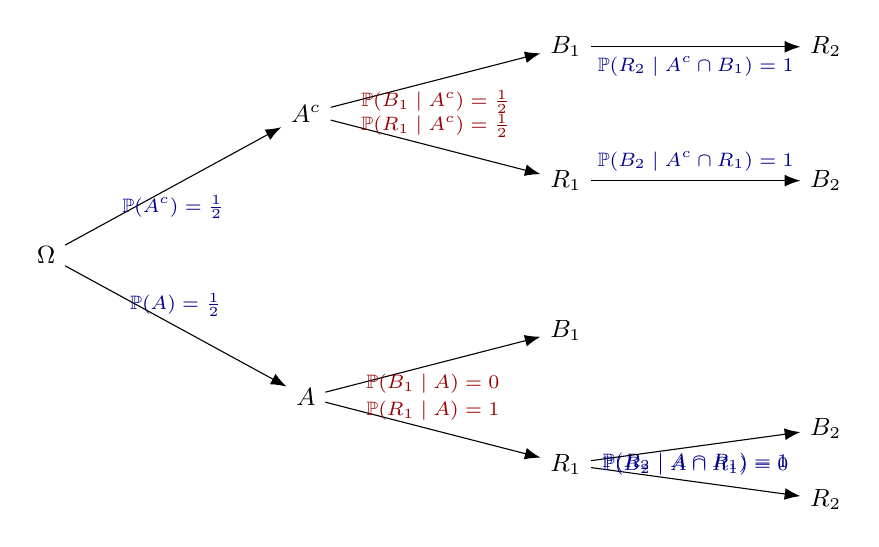
\begin{tikzpicture}[albero]
\node {$\Omega$}
  child { node {$A$}
    child { node {$R_1$}
      child { node {$R_2$} edge from parent node[etichetta]{$\mathbb{P}(R_2\mid A\cap R_1)=1$} }
      child { node {$B_2$} edge from parent node[etichetta,below]{$\mathbb{P}(B_2\mid A\cap R_1)=0$} }
      edge from parent node[etichettaR]{$\mathbb{P}(R_1\mid A)=1$}
    }
    child { node {$B_1$} edge from parent node[etichettaR,below]{$\mathbb{P}(B_1\mid A)=0$} }
    edge from parent node[etichetta]{$\mathbb{P}(A)=\frac12$}
  }
  child { node {$A^c$}
    child { node {$R_1$}
      child { node {$B_2$} edge from parent node[etichetta]{$\mathbb{P}(B_2\mid A^c\cap R_1)=1$} }
      edge from parent node[etichettaR]{$\mathbb{P}(R_1\mid A^c)=\frac12$}
    }
    child { node {$B_1$}
      child { node {$R_2$} edge from parent node[etichetta,below]{$\mathbb{P}(R_2\mid A^c\cap B_1)=1$} }
      edge from parent node[etichettaR,below]{$\mathbb{P}(B_1\mid A^c)=\frac12$}
    }
    edge from parent node[etichetta,below]{$\mathbb{P}(A^c)=\frac12$}
  };
\end{tikzpicture}
\end{center}

\emph{Lettura del disegno:} il cammino $\Omega\to A\to R_1\to R_2$ ha probabilit\`a $\frac12\cdot1\cdot1=\frac12$; l'evento ``esce $R_2$'' \`e dato dai due cammini che finiscono in $R_2$ (via $A\cap R_1$ e via $A^c\cap B_1$), quindi $P(R_2)=\frac12\cdot1\cdot1+\frac12\cdot\frac12\cdot1=\frac34$.
\end{concetto}

\begin{concetto}{Indipendenza}
\inparole{$A$ e $B$ sono indipendenti se sapere che uno \`e accaduto non cambia la probabilit\`a dell'altro.}
\[ A, B \text{ indipendenti} \iff P(A \cap B) = P(A)\, P(B) \]
Equivale a $P(A \mid B) = P(A)$. Per $n$ eventi indipendenti: $P(A_1 \cap \cdots \cap A_n) = P(A_1)\cdots P(A_n)$.
\end{concetto}

\begin{attenzione}
Incompatibili $\neq$ indipendenti! Se $A \cap B = \emptyset$ con $P(A),P(B)>0$, allora $P(A\cap B)=0 \neq P(A)P(B)$: sono \emph{dipendenti} (se accade uno, l'altro \`e escluso).
\end{attenzione}

\begin{concetto}{Prove ripetute indipendenti e formula del binomio}
Ripeto $n$ volte una prova indipendente con probabilit\`a $p$ di successo. La probabilit\`a di \textbf{esattamente $k$ successi} \`e:
\[ P(k \text{ successi su } n) = \binom{n}{k} p^k (1-p)^{n-k} \]
\textbf{Attenzione a non confondere:}
\begin{itemize}[leftmargin=1.2em,itemsep=1pt,topsep=2pt]
\item una \emph{sequenza specifica} di $k$ successi $\Rightarrow$ solo $p^k(1-p)^{n-k}$;
\item $k$ successi \emph{in ordine qualsiasi} $\Rightarrow$ si aggiunge $\binom{n}{k}$.
\end{itemize}
\end{concetto}

\begin{trucco}
\textbf{Riconoscimento:} categorie (rischio basso/alto, urne, cavalieri/furfanti\dots), condizionali, domande ``sapendo che\dots''.

\textbf{Passi (tipo 1):}
\begin{enumerate}[leftmargin=1.4em,itemsep=1pt,topsep=2pt]
\item Definire la partizione $E_1,\dots,E_n$ e l'evento $A$; scrivere $P(E_i)$ e $P(A\mid E_i)$.
\item $P(A) = \sum_i P(A\mid E_i)P(E_i)$ (probabilit\`a totali).
\item Se chiede ``sapendo $A$\dots'': Bayes $P(E_j\mid A)$.
\item Due eventi indipendenti: moltiplica. Unione: $P(A\cup B)=P(A)+P(B)-P(A\cap B)$.
\item $k$ successi su $n$ prove indipendenti: binomio.
\item Se l'esperimento ha pi\`u fasi in sequenza: conviene \textbf{disegnare l'albero} (v. box sopra), moltiplicare lungo i rami e sommare le foglie che interessano.
\end{enumerate}
\end{trucco}

% ======================================================
\newpage
\section{Variabili Aleatorie Discrete}

\begin{concetto}[barBlue]{Determinare $(\Omega, P)$ per un esperimento aleatorio}
\inparole{$\Omega$ \`e l'insieme di tutti i possibili esiti elementari dell'esperimento; $P$ \`e la regola che assegna una probabilit\`a a ciascun esito (o evento).}

\textbf{Passi per costruire $(\Omega, P)$:}
\begin{enumerate}[leftmargin=1.4em,itemsep=2pt,topsep=2pt]
\item \textbf{Identificare l'esperimento elementare}: cosa viene effettivamente osservato/estratto/lanciato (es.\ un dado, una pallina, un lancio di moneta).
\item \textbf{Definire $\Omega$}: l'insieme di \emph{tutti} gli esiti possibili, elementari e mutuamente esclusivi.
\begin{itemize}[leftmargin=1.2em,itemsep=1pt,topsep=1pt]
\item Se ci sono pi\`u prove/estrazioni, $\Omega$ \`e tipicamente un prodotto cartesiano: $\Omega=\{1,\dots,6\}^2$ (due dadi), oppure sequenze ordinate $\Omega=\{(a_1,\dots,a_n)\}$.
\item Attenzione a \textbf{ordine} e \textbf{ripetizione}: estrazioni con/senza reinserimento, ordinate/non ordinate cambiano la cardinalit\`a di $\Omega$.
\end{itemize}
\item \textbf{Assegnare $P$ sugli esiti elementari}:
\begin{itemize}[leftmargin=1.2em,itemsep=1pt,topsep=1pt]
\item Se gli esiti sono \textbf{equiprobabili} (dadi non truccati, palline indistinguibili estratte a caso): $P(\omega) = \dfrac{1}{|\Omega|}$ per ogni $\omega$, e per un evento $A$: $P(A) = \dfrac{|A|}{|\Omega|}$ (calcolo combinatorio).
\item Se gli esiti \textbf{non} sono equiprobabili, assegnare $P(\omega)$ singolarmente in base ai dati del problema (es.\ moneta truccata con $P(\text{testa})=p$).
\end{itemize}
\item \textbf{Verificare gli assiomi}: $P(\omega) \ge 0$ per ogni $\omega$, e $\displaystyle\sum_{\omega \in \Omega} P(\omega) = 1$.
\item \textbf{Esprimere gli eventi di interesse come sottoinsiemi di $\Omega$}: un evento $A$ \`e un insieme di esiti, $A \subseteq \Omega$, e $P(A) = \sum_{\omega \in A} P(\omega)$.
\end{enumerate}
\end{concetto}

\begin{trucco}
\textbf{Riconoscimento:} qualunque problema che descrive un esperimento fisico (lanci, estrazioni, code, guasti) va \emph{sempre} tradotto per primo in $(\Omega,P)$ esplicito, anche se poi si useranno v.a.\ per semplificare i calcoli.

\textbf{Errore comune:} confondere $\Omega$ (esiti elementari) con il \textbf{supporto} di una v.a.\ $X$ definita su $\Omega$ -- sono due insiemi diversi collegati da $X:\Omega\to\mathbb{R}$.

\textbf{Esempio minimo:} lancio due dadi equi. $\Omega=\{(i,j): i,j\in\{1,\dots,6\}\}$, $|\Omega|=36$, $P(\omega)=\tfrac{1}{36}$ per ogni $\omega$. Evento $A=$``somma $=7$'' $\Rightarrow A=\{(1,6),(2,5),\dots,(6,1)\}$, $|A|=6$, $P(A)=\tfrac{6}{36}=\tfrac{1}{6}$.
\end{trucco}

\begin{concetto}[barBlue]{Cos'\`e una variabile aleatoria}
\inparole{una variabile aleatoria (v.a.) $X$ \`e un \emph{numero} che dipende dall'esito: una funzione $X:\Omega \to \mathbb{R}$.}

\`E \textbf{discreta} se assume valori isolati (finiti o numerabili: $0,1,2,\dots$).

\emph{Esempio:} lancio due dadi, $\Omega=\{1,\dots,6\}^2$. Definisco $X(i,j)=i+j$ (somma) e $Y(i,j)=\max(i,j)$: sono v.a.\ costruite sugli esiti.
\end{concetto}

\begin{concetto}[barBlue]{Densit\`a e funzione di ripartizione (caso discreto)}
\begin{itemize}[leftmargin=1.2em,itemsep=2pt,topsep=2pt]
\item \textbf{Densit\`a} (o legge): $p_X(k) = P(X=k)$, con $p_X(k)\ge 0$ e $\sum_k p_X(k)=1$.
\item \textbf{Funzione di ripartizione}: $F_X(x) = P(X \le x) = \sum_{k \le x} p_X(k)$ (a gradini, cresce da 0 a 1).
\item $P(a < X \le b) = F_X(b) - F_X(a)$.
\item \textbf{Attenzione a $<$ vs $\le$} (nel discreto \emph{contano}, perch\'e $P(X=k)>0$): $\ P(a \le X \le b) = F_X(b) - F_X(a^-)$, dove $F_X(a^-)$ \`e il valore ``appena prima'' di $a$ (esclude il salto in $a$). Cio\`e $P(a\le X\le b)$ e $P(a<X\le b)$ differiscono di $P(X=a)$.
\item \textbf{Coda destra:} $P(X > x) = 1 - P(X \le x)$.
\end{itemize}
\end{concetto}

\begin{concetto}[barBlue]{Valore atteso e varianza}
\inparole{$E[X]$ \`e la media ``pesata'' dei valori; $\mathrm{Var}(X)$ misura quanto $X$ si disperde attorno alla media.}
\[ E[X] = \sum_{k} k\, p_X(k), \qquad E[g(X)] = \sum_{k} g(k)\, p_X(k) \]
\[ \mathrm{Var}(X) = E[X^2] - (E[X])^2, \qquad \sigma_X = \sqrt{\mathrm{Var}(X)} \]
\textbf{Propriet\`a:} $E[aX+b]=aE[X]+b$; \; $\mathrm{Var}(aX+b)=a^2\mathrm{Var}(X)$; \; $E[X+Y]=E[X]+E[Y]$ (sempre).
\end{concetto}

\begin{concetto}[barBlue]{Distribuzioni discrete notevoli}
\begin{center}\small
\begin{tabular}{lcccccc}
\hline
Distribuzione & Parametri & Densit\`a $p_X(k)$ & Supporto & $E[X]$ & $\mathrm{Var}(X)$ \\
\hline
Bernoulli $\mathrm{Be}(p)$ & $p \in (0,1)$ & $p^k(1-p)^{1-k}$ & $\{0,1\}$ & $p$ & $p(1-p)$ \\[6pt]
Binomiale $\mathrm{Bin}(n,p)$ & $n,\ p \in (0,1)$ & $\binom{n}{k}p^k(1-p)^{n-k}$ & $\{0,\dots,n\}$ & $np$ & $np(1-p)$ \\[6pt]
Geometrica $\mathrm{Geo}(p)$ & $p \in (0,1)$ & $(1-p)^{k-1}p$ & $\{1,2,\dots\}$ & $\dfrac{1}{p}$ & $\dfrac{1-p}{p^2}$ \\[10pt]
Poisson $\mathrm{Po}(\lambda)$ & $\lambda>0$ & $e^{-\lambda}\dfrac{\lambda^k}{k!}$ & $\{0,1,2,\dots\}$ & $\lambda$ & $\lambda$ \\[10pt]
Ipergeom.\ $\mathrm{H}(N,K,n)$ & $N,K,n$ & $\dfrac{\binom{K}{k}\binom{N-K}{n-k}}{\binom{N}{n}}$ & $k$ ammissibili & $n\dfrac{K}{N}$ & $n\dfrac{K}{N}\dfrac{N-K}{N}\dfrac{N-n}{N-1}$ \\[6pt]
\hline
\end{tabular}
\end{center}
\small \textbf{Quando usarle:} Bernoulli = una prova (successo/insuccesso); Binomiale = n.\ di successi su $n$ prove \emph{con} reinserimento; Ipergeometrica = n.\ di successi su $n$ estrazioni \emph{senza} reinserimento; Geometrica = n.\ di prove fino al primo successo; Poisson = conteggi di eventi rari nel tempo/spazio.

\textbf{Coda destra (complementare):} per distribuzioni illimitate ($\{0,1,2,\dots\}$) non si sommano infiniti termini; si passa al complementare. Es.\ $N\sim\mathrm{Po}(\lambda)$:
\[ P(N > 2) = 1 - P(N{=}0) - P(N{=}1) - P(N{=}2) = 1 - e^{-\lambda}\!\left(1+\lambda+\tfrac{\lambda^2}{2}\right) \]
In generale $P(N>m)=1-\sum_{k=0}^{m}P(N{=}k)$ \; (``$>m$'' esclude $m$, ``$\ge m$'' lo include).
\end{concetto}

\begin{concetto}[barBlue]{Vettori: densit\`a congiunta e marginali}
$(X,Y)$ vettore aleatorio discreto. Il \textbf{supporto} sono le coppie con probabilit\`a $>0$:
\[ \text{Supporto} = \{(x,y): p_{(X,Y)}(x,y)>0\} = \{(x_1,y_1),(x_2,y_2),\dots\} \]
\begin{itemize}[leftmargin=1.2em,itemsep=2pt,topsep=2pt]
\item Densit\`a congiunta: $p_{(X,Y)}(x,y) = P(X{=}x, Y{=}y)$.
\item Marginale di $X$: $p_X(x) = \sum_{y} p_{(X,Y)}(x,y)$ (somma per colonne).
\item Marginale di $Y$: $p_Y(y) = \sum_{x} p_{(X,Y)}(x,y)$ (somma per righe).
\item Controllo: $\sum_{x,y} p_{(X,Y)}(x,y) = 1$.
\end{itemize}
\end{concetto}

\begin{concetto}[barBlue]{Covarianza, correlazione e varianza di una somma}
\[ \mathrm{Cov}(X,Y) = E[XY] - E[X]E[Y], \qquad E[XY] = \sum_{x,y} xy\, p_{(X,Y)}(x,y) \]
\[ \rho(X,Y) = \frac{\mathrm{Cov}(X,Y)}{\sigma_X \sigma_Y} \in [-1,1], \qquad \mathrm{Var}(X+Y) = \mathrm{Var}(X)+\mathrm{Var}(Y)+2\mathrm{Cov}(X,Y) \]
\textbf{Propriet\`a:} $\mathrm{Cov}(X,X)=\mathrm{Var}(X)$; \; $\mathrm{Cov}(aX,bY)=ab\,\mathrm{Cov}(X,Y)$; \; $\mathrm{Cov}(X{+}Z,Y)=\mathrm{Cov}(X,Y)+\mathrm{Cov}(Z,Y)$.
\end{concetto}

\begin{concetto}[barBlue]{Indipendenza discreta}
$X$ e $Y$ indipendenti $\iff p_{(X,Y)}(x,y) = p_X(x)\,p_Y(y)$ per ogni $x,y$.

Conseguenza: se $X \perp Y$ allora $\mathrm{Cov}(X,Y)=0$.
\end{concetto}

\begin{attenzione}
Il viceversa \`e \textbf{FALSO}: $\mathrm{Cov}(X,Y)=0 \not\Rightarrow$ indipendenza. Per provare la \emph{non}-indipendenza basta \emph{un} caso $(x_0,y_0)$ con $p_{(X,Y)}(x_0,y_0) \neq p_X(x_0)p_Y(y_0)$.
\end{attenzione}

\begin{concetto}[barBlue]{Legge di una trasformazione $Z=g(X,Y)$}
\begin{enumerate}[leftmargin=1.4em,itemsep=1pt,topsep=2pt]
\item Supporto $S_Z = \{g(x,y):(x,y)\in\text{supp}\}$.
\item Per ogni $z$: $\ p_Z(z) = \sum_{\{(x,y):g(x,y)=z\}} p_{(X,Y)}(x,y)$.
\end{enumerate}
Casi tipici: $Z=X+Y \Rightarrow p_Z(z)=\sum_x p_{(X,Y)}(x,z-x)$; \; $W=X-Y \Rightarrow p_W(w)=\sum_x p_{(X,Y)}(x,x-w)$.
\end{concetto}

\begin{concetto}[barBlue]{Probabilit\`a di un evento su $(X,Y)$}
Per calcolare $P$ di un evento descritto da $X,Y$ (es. $P(X\ge Y)$, $P(U\ge V)$, $P(X=Y)$): si \textbf{sommano le celle della congiunta} che soddisfano la condizione.
\[ P\big((X,Y)\in A\big) = \sum_{(x,y)\in A} p_{(X,Y)}(x,y) \]
Es.\ $P(X\ge Y)=\sum_{x\ge y} p_{(X,Y)}(x,y)$. Spesso l'evento si semplifica prima algebricamente: es.\ $(X{-}1)Y \ge X(Y{-}1) \iff X\ge Y$.
\end{concetto}

\begin{concetto}[barBlue]{Minimo e massimo di due v.a.\ indipendenti}
Se $X \perp Y$, conviene passare per la ripartizione (vale sia nel discreto sia nel continuo):
\[ W=\max(X,Y):\quad F_W(t)=P(X\le t,\,Y\le t)=F_X(t)\,F_Y(t) \]
\[ Z=\min(X,Y):\quad P(Z> t)=P(X>t)\,P(Y>t) \ \Rightarrow\ F_Z(t)=1-\big(1-F_X(t)\big)\big(1-F_Y(t)\big) \]
\emph{Idea:} ``il max $\le t$'' vuol dire \emph{entrambi} $\le t$; ``il min $>t$'' vuol dire \emph{entrambi} $>t$. Nel discreto si ricava poi $p_W$/$p_Z$ per differenza; per la \textbf{congiunta} di $(\min,\max)$ si distinguono i casi $z<w$, $z=w$, $z>w$.
\end{concetto}

\begin{trucco}
\textbf{Riconoscimento:} dadi, monete, palline, tabella di probabilit\`a congiunta.

\textbf{Passi (tipo 2):}
\begin{enumerate}[leftmargin=1.4em,itemsep=1pt,topsep=2pt]
\item Costruire $(\Omega,P)$; definire le v.a.\ come funzioni sugli esiti.
\item Tabella della congiunta; ricavare le marginali (somme di riga/colonna).
\item $E[X],E[Y],E[XY]$, poi $\mathrm{Cov}=E[XY]-E[X]E[Y]$.
\item Indipendenza: test $p_{(X,Y)}=p_X\cdot p_Y$ (o controesempio).
\item Trasformazioni $Z=g(X,Y)$: costruire la nuova tabella sommando le celle.
\end{enumerate}
\end{trucco}

% ======================================================
\newpage
\section{Variabili Aleatorie Continue}

\begin{concetto}[barGreen]{Densit\`a e funzione di ripartizione}
\inparole{una v.a.\ \`e \emph{continua} se pu\`o assumere tutti i valori di un intervallo; la ``densit\`a'' $f_X$ non \`e una probabilit\`a ma un peso, e la probabilit\`a \`e l'\emph{area} sotto $f_X$.}
\begin{itemize}[leftmargin=1.2em,itemsep=2pt,topsep=2pt]
\item Normalizzazione: $\int_{-\infty}^{+\infty} f_X(x)\,dx = 1$, con $f_X(x)\ge 0$.
\item Ripartizione: $F_X(x) = P(X \le x) = \int_{-\infty}^{x} f_X(t)\,dt$; \; inversa: $f_X(x)=F_X'(x)$.
\item $P(a<X\le b) = F_X(b)-F_X(a) = \int_a^b f_X(x)\,dx$.
\item \textbf{Caso continuo --- $<$ e $\le$ sono equivalenti} (perch\'e $P(X=a)=0$):
\[ P(a<X<b) = P(a\le X\le b) = P(a<X\le b) = P(a\le X<b) = F_X(b)-F_X(a) \]
\item Prob.\ puntuale (utile nel caso misto): $P(X=x) = F_X(x) - F_X(x^-)$. Se $X$ \`e continua vale $0$.
\end{itemize}
\end{concetto}

\begin{attenzione}
L'equivalenza $<\,\Leftrightarrow\,\le$ vale \textbf{solo nel caso continuo}. Per una v.a.\ \textbf{discreta} (o mista) i punti hanno probabilit\`a $>0$, quindi includere o no l'estremo cambia il risultato:
\[ P(a<X\le b) = F_X(b)-F_X(a), \qquad P(a\le X\le b) = F_X(b)-F_X(a^-) \]
(differiscono di $P(X=a)$).
\end{attenzione}

\begin{concetto}[barGreen]{Trovare $f_X$ data $F_X$ (operazione inversa)}
\`E il contrario della ripartizione: la densit\`a \`e la \textbf{derivata} della funzione di ripartizione.
\[ \boxed{\ f_X(x) = F_X'(x)\ } \]
Se $F_X$ \`e definita \textbf{a tratti}, si deriva ogni pezzo separatamente (e vale $0$ dove $F_X$ \`e costante):
\[ F_X(x)=\begin{cases}\dots \\ F_1(x) & a\le x\le b \\ F_2(x) & b< x\le c \\ \dots\end{cases} \ \Longrightarrow\ f_X(x)=\begin{cases}0 & \text{dove }F_X \text{ costante} \\ F_1'(x) & a\le x\le b \\ F_2'(x) & b< x\le c \\ 0 & \text{altrove}\end{cases} \]
\emph{Controllo:} $f_X\ge0$ e $\int f_X = 1$ (equivale a $F_X(+\infty)=1$, $F_X(-\infty)=0$). Nei punti d'angolo di $F_X$ la derivata pu\`o non esistere: l\`i il valore di $f_X$ \`e irrilevante (insieme di misura nulla).

\emph{Esempio (triangolare):} da $F_X(x)=\frac{x^2}{2}$ su $[0,1]$ e $2x-\frac{x^2}{2}-1$ su $(1,2]$ si deriva $f_X(x)=x$ su $[0,1]$, $f_X(x)=2-x$ su $(1,2]$, $0$ altrove.
\end{concetto}

\begin{concetto}[barGreen]{Verificare che $f_X$ \`e una densit\`a}
La verifica principale \`e che l'\textbf{integrale (area totale) faccia 1}:
\[ \boxed{\ \int_{-\infty}^{+\infty} f_X(x)\,dx = 1\ } \]
(insieme alla condizione di base $f_X(x) \ge 0$ per ogni $x$). Per una densit\`a \textbf{a tratti} l'integrale \`e la somma degli integrali sui singoli pezzi. Se il risultato $\neq 1$: o c'\`e una costante $c$ da determinare imponendo $\int f = 1$, oppure la funzione non \`e una densit\`a.
\end{concetto}

\begin{concetto}[barGreen]{Ripartizione $F_X$ da una densit\`a a tratti (metodo)}
$F_X(x)=P(X\le x)=\int_{-\infty}^{x} f(t)\,dt$ si costruisce intervallo per intervallo, \textbf{accumulando l'area}.
\begin{enumerate}
\item Prima del supporto: $F_X(x)=0$.
\item Primo pezzo $[a_0,a_1]$: $\ F_X(x)=\displaystyle\int_{a_0}^{x} f(t)\,dt$.
\item Pezzo successivo $[a_1,a_2]$: si \emph{riparte dal valore gi\`a accumulato} $F_X(a_1)$ (= il pezzo precedente valutato nel suo estremo destro) e si aggiunge l'integrale sul nuovo pezzo:
\[ F_X(x)=F_X(a_1)+\int_{a_1}^{x} f(t)\,dt \]
(si ripete per ogni pezzo successivo, sempre ripartendo dal valore accumulato).
\item Dopo il supporto: $F_X(x)=1$.
\item \textbf{Controllo finale:} $F_X$ deve venire \textbf{continua} e crescente da $0$ a $1$.
\end{enumerate}
\emph{In pratica:} l'estremo sinistro del nuovo pezzo, messo nella formula del pezzo precedente, d\`a la costante di partenza.

\textbf{Esempio (triangolare):} $f(x)=x$ su $[0,1]$, $\ f(x)=2-x$ su $(1,2]$, $\ 0$ altrove.
\begin{itemize}[leftmargin=1.2em,itemsep=1pt,topsep=2pt]
\item \emph{Verifica densit\`a:} $\int_0^1 x\,dx + \int_1^2 (2-x)\,dx = \tfrac12+\tfrac12 = 1$ \checkmark \; (e $f\ge0$).
\item $0\le x\le1$: $\ F_X(x)=\int_0^x t\,dt = \dfrac{x^2}{2}$; \; in $x=1$ vale $\tfrac12$.
\item $1<x\le2$: $\ F_X(x)=\dfrac12+\int_1^x (2-t)\,dt = 2x-\dfrac{x^2}{2}-1$; \; in $x=2$ vale $1$.
\end{itemize}
\[ F_X(x)=\begin{cases} 0 & x<0 \\[2pt] \dfrac{x^2}{2} & 0\le x\le 1 \\[4pt] 2x-\dfrac{x^2}{2}-1 & 1<x\le 2 \\[4pt] 1 & x>2 \end{cases} \]
\end{concetto}

\begin{concetto}[barGreen]{Valore atteso, varianza}
\[ E[X] = \int_{-\infty}^{+\infty} x\,f_X(x)\,dx, \quad E[X^2] = \int_{-\infty}^{+\infty} x^2 f_X(x)\,dx, \quad \mathrm{Var}(X) = E[X^2]-(E[X])^2 \]
\end{concetto}

\begin{concetto}[barGreen]{Metodo generale: legge di $Y=g(X)$}
Su $S_X=[p,q]$, $S_Y=[\min_{x\in S_X} g(x),\ \max_{x\in S_X} g(x)]$.
\begin{enumerate}
\item Calcolare (se non lo si ha gia') $F_X(x) =  \begin{cases}
0 \quad & x < p \\
\int_{p}^x f_x(t) \, dt \quad & x \in [p,q]\\
1 \quad & x \geq q
  \end{cases}$
\item $F_Y(y)=0 \quad y < \min g \qquad F_Y(y)=1 \quad y \geq \max g$
\item Per $y$ nel range di $S_Y$, isolare $X$ nella disuguaglianza $g(X)\le y$.
\begin{itemize}
\item se $g$ \`e \textbf{monotona} su $S_X$ (crescente o decrescente), la condizione $g(X)\le y$ ha un solo lato: $X\le g^{-1}(y)$ (crescente, $F_Y=F_X(g^{-1}(y))$) oppure $X\ge g^{-1}(y)$ (decrescente, la disuguaglianza si ribalta, $F_Y=1-F_X(g^{-1}(y))$), \textbf{per ogni} $y\in S_Y$.
\item se $g$ \textbf{non \`e monotona} (es.\ $X^2$, $|X-a|$): la condizione si spezza in \textbf{due lati}, $h_1(y)\le X\le h_2(y)$. Esiste una soglia $y^*\in S_Y$ in cui uno dei due bordi $h_1(y)$, $h_2(y)$ esce da $S_X=[p,q]$ (cio\`e $F_X$ vale gi\`a $0$ o $1$ l\`i): per $y<y^*$ (nessun bordo satura) $F_Y(y)=F_X(h_2(y))-F_X(h_1(y))$; per $y\ge y^*$ (un bordo saturo) resta solo l'altro pezzo.
\end{itemize}
Quindi, nel caso non monotono, in generale
\[ F_Y(y)= \begin{cases}
0 & y < \min g\\
F_X(h_2(y))-F_X(h_1(y)) & y\in[\min g,\, y^*)\\
F_X(h_2(y))\ \text{oppure}\ 1-F_X(h_1(y)) & y\in[y^*,\, \max g)\\
1 & y \geq \max g
\end{cases} \]
(vedi i box specifici per $Y=X^2$ e $Y=|X-a|$ per l'individuazione concreta di $y^*$).
\item Infine calcoliamo $f_Y(y)=F_Y'(y)$ derivando ogni pezzo separatamente (regola della catena: $\big(F_X(h(y))\big)'=h'(y)\,f_X(h(y))$):
\[ f_Y(y) = \begin{cases}
0 \quad & y < \min g \lor y \geq \max g\\
h_2'(y)\,f_X(h_2(y)) - h_1'(y)\,f_X(h_1(y)) \quad & y \in [\min g,\, y^*)\\
\text{derivata del pezzo restante} \quad & y \in [y^*,\, \max g)
\end{cases} \]
Controllo: $f_Y\ge0$, $\int f_Y=1$.
\end{enumerate}
\end{concetto}

\begin{concetto}[barGreen]{Svolgere $P(g(X)\le y)$: isolare $X$ (casi comuni)}
Il cuore del metodo \`e trasformare $g(X)\le y$ in una condizione su $X$. Regola:
\begin{itemize}[leftmargin=1.2em,itemsep=1pt,topsep=2pt]
\item $g$ \textbf{crescente} $\Rightarrow$ $X\le g^{-1}(y)$, quindi $F_Y(y)=F_X(g^{-1}(y))$;
\item $g$ \textbf{decrescente} $\Rightarrow$ la disuguaglianza \emph{si ribalta}: $X\ge g^{-1}(y)$, quindi $F_Y(y)=1-F_X(g^{-1}(y))$;
\item $g$ \textbf{non monotona} ($X^2$, $|X|$) $\Rightarrow$ condizione a due lati.
\end{itemize}
\renewcommand{\arraystretch}{1.8}
\begin{center}
\begin{tabular}{c|c|c}
$Y=g(X)$ & $g(X)\le y \iff$ & $F_Y(y)=$ \\
\hline
$cX\ (c>0)$ & $X\le \dfrac{y}{c}$ & $F_X\!\big(\tfrac{y}{c}\big)$ \\
$cX\ (c<0)$ & $X\ge \dfrac{y}{c}$ (ribalta) & $1-F_X\!\big(\tfrac{y}{c}\big)$ \\
$aX+b\ (a>0)$ & $X\le \dfrac{y-b}{a}$ & $F_X\!\big(\tfrac{y-b}{a}\big)$ \\
$X^3$ & $X\le \sqrt[3]{y}$ & $F_X\!\big(\sqrt[3]{y}\big)$ \\
$e^{X}$ & $X\le \ln y\ (y>0)$ & $F_X(\ln y)$ \\
$\sqrt{X}$ & $X\le y^2\ (y\ge0)$ & $F_X(y^2)$ \\
$c(1-X)\ (c>0)$ & $X\ge \dfrac{c-y}{c}$ (ribalta) & $1-F_X\!\big(\tfrac{c-y}{c}\big)$ \\
$X^2$ & $-\sqrt{y}\le X\le \sqrt{y}\ (y\ge0)$ & $F_X(\sqrt{y})-F_X(-\sqrt{y})$ \\
$|X|$ & $-y\le X\le y\ (y\ge0)$ & $F_X(y)-F_X(-y)$ \\
\end{tabular}
\end{center}
\renewcommand{\arraystretch}{1}
\emph{Attenzione al ribaltamento:} ogni volta che dividi per un numero negativo o applichi una funzione decrescente, il verso della disuguaglianza si inverte ($\le$ diventa $\ge$).
\end{concetto}

\begin{concetto}[barGreen]{Determinare la legge della variabile aleatoria $Y=X^2$}
Su $S_X=[-a,b]$, $S_Y=[0,\max(a^2,b^2)]$. 
\begin{enumerate}
\item Calcolare (se non lo si ha gia') $F_X(x) =  \begin{cases}
0 \quad & x < (-a) \\
\int_{(-a)}^x f_x(t) \, dt \quad & x \in [-a,b]\\
1 \quad & x \geq b
  \end{cases}$ 
\item $F_Y(y)=0 \quad y < 0 \qquad F_Y(y)=1 \quad y \geq \max(a^2,b^2)$
\item Per $y\in[0,a^2)$:
\[ F_Y(y)=P(-\sqrt{y}\le X\le\sqrt{y})=F_X(\sqrt{y})-F_X(-\sqrt{y}) \]
Altrimenti $y \in [a^2, \max(a^2,b^2))$
\begin{align*}
  F_Y(y)=P(X\le\sqrt{y})=F_X(\sqrt{y})
\end{align*}
Quindi avremo
\begin{align*}
  F_Y(y)= \begin{cases}
    0 & y < 0\\
    F_X(\sqrt{y})-F_X(-\sqrt{y}) & y\in[0,a^2)\\
    F_X(\sqrt{y}) &y \in [a^2, \max(a^2,b^2))\\
    1 & y \geq \max(a^2,b^2)
  \end{cases}
\end{align*}
\item Infine calcoliamo 
\begin{align*}
  f_Y(y) = \begin{cases}
0 \quad & y < 0 \land y \geq \max(a^2,b^2)\\
    \dfrac{d(F_X(\sqrt{y})-F_X(-\sqrt{y}))}{dy} \quad & y \in [0, a^2]\\
    \dfrac{d(F_X(\sqrt{y}))}{dy} \quad & \text{ nel restante}
\end{cases}
\end{align*}
\end{enumerate}
\end{concetto}

\begin{concetto}[barGreen]{Caso $Y=|X-a|$ (valore assoluto)}
Su $S_X=[p,q]$ (con $a\in[p,q]$), $Y=|X-a|\ge0$, $S_Y=[0,\max(a-p,\,q-a)]$.
\begin{enumerate}
\item Calcolare (se non lo si ha gia') $F_X(x) =  \begin{cases}
0 \quad & x < p \\
\int_{p}^x f_x(t) \, dt \quad & x \in [p,q]\\
1 \quad & x \geq q
  \end{cases}$

\item $F_Y(y)=0 \quad y < 0 \qquad F_Y(y)=1 \quad y \geq \max(a-p,\,q-a)$

\item Per $y\ge0$ togliamo il modulo: $|X-a|\le y \iff a-y\le X\le a+y$. La \textbf{cases} nasce da come $[a-y,a+y]$ interseca $S_X=[p,q]$: il bordo sinistro $a-y$ esce da $S_X$ quando $y\ge a-p$, il bordo destro $a+y$ esce quando $y\ge q-a$. Sia $m=\min(a-p,\,q-a)$, $M=\max(a-p,\,q-a)$.

Per $y\in[0,m)$ (nessun bordo satura):
\[ F_Y(y)=P(a-y\le X\le a+y)=F_X(a+y)-F_X(a-y) \]

Per $y\in[m,M)$ (un bordo satura — dipende da chi tra $a-p$ e $q-a$ è più piccolo):
\[
F_Y(y)=
\begin{cases}
F_X(a+y) & \text{se } m=a-p \ \ (\text{cio\`e } F_X(a-y)=0)\\
1-F_X(a-y) & \text{se } m=q-a \ \ (\text{cio\`e } F_X(a+y)=1)
\end{cases}
\]

Quindi avremo
\begin{align*}
  F_Y(y)= \begin{cases}
    0 & y < 0\\
    F_X(a+y)-F_X(a-y) & y\in[0,m)\\
    F_X(a+y) \ \text{oppure} \ 1-F_X(a-y) & y \in [m, M)\\
    1 & y \geq M
\end{cases}
\end{align*}

\item Infine calcoliamo
\begin{align*}
  f_Y(y) = \begin{cases}
0 \quad & y < 0 \lor y \geq M\\
    f_X(a+y)+f_X(a-y) \quad & y \in [0, m)\\
    f_X(a+y) \ \text{oppure} \ f_X(a-y) \quad & y \in [m,M)
\end{cases}
\end{align*}

\emph{Esempio} ($X$ triangolare su $[0,2]$, $a=1$): qui $p=0,q=2$, quindi $a-p=1=q-a=1$, cio\`e $m=M=1$ (caso simmetrico, non serve la fascia intermedia). Con la $F_X$ trovata prima,
\[ F_Y(y)=F_X(1+y)-F_X(1-y) = 2y - y^2 \ \ (0\le y\le1) \qquad f_Y(y)=2-2y \]
\[ F_Y(y)=\begin{cases} 0 & y<0 \\ 2y-y^2 & 0\le y\le 1 \\ 1 & y>1 \end{cases} \]
\end{enumerate}
\end{concetto}

\begin{concetto}[barGreen]{Distribuzioni miste (n\'e continue n\'e discrete)}
Alcune trasformazioni danno una v.a.\ \textbf{mista}: la ripartizione $F$ \`e in parte continua e in parte ``a salti''. Nasce quando $g$ \emph{schiaccia} un pezzo di $X$ su un punto (es.\ $\min(X,c)$) o quando si mescola con una Bernoulli (es.\ $Z=TX$ con $T\sim\mathrm{Be}(p)$).
\begin{itemize}[leftmargin=1.2em,itemsep=2pt,topsep=2pt]
\item \textbf{Salto di $F$ in $x$} $\Rightarrow$ atomo: $P(X=x)=F_X(x)-F_X(x^-) > 0$.
\item \textbf{Non \`e continua} se $F$ ha almeno un salto.
\item \textbf{Non \`e discreta} se la somma di tutti i salti \`e $<1$ (c'\`e anche una parte ``liscia''): $\sum_x \big(F(x)-F(x^-)\big) < 1$.
\end{itemize}
\textbf{Come si calcola $F_Z$} per una mista tipo $Z=TX$: si condiziona su $T$ (probabilit\`a totali):
\[ F_Z(z)=P(Z\le z)=P(T{=}0)\,P(0\le z) + P(T{=}1)\,P(X\le z) \]
\emph{Caso $\min(X,c)$:} per $t<c$ vale $F(t)=F_X(t)$; in $t=c$ compare un atomo $P(=c)=P(X\ge c)$ (tutta la coda si accumula su $c$). Se $c$ \`e sotto il supporto di $X$, $\min(X,c)=c$ \`e \textbf{degenere} ($\mathbb{P}=\delta_c$).
\end{concetto}

\begin{concetto}[barGreen]{Trasformazione lineare $Y=aX+b$ e $Z=\frac{X-c}{d}$}
\[ f_Y(y) = \frac{1}{|a|}f_X\!\left(\frac{y-b}{a}\right), \qquad F_Y(y)=F_X\!\left(\frac{y-b}{a}\right)\ (a>0) \]
Per $Z=\frac{X-c}{d}$ scrivi $a=\frac1d$, $b=-\frac cd$. Media e varianza (per qualsiasi $X$):
\[ E[Z]=\frac{E[X]-c}{d}, \qquad \mathrm{Var}(Z)=\frac{\mathrm{Var}(X)}{d^2}, \qquad f_Z(z)=d\,f_X(dz+c) \]
Se $X\sim\mathcal{N}(\mu,\sigma^2)$ resta normale: $Z\sim\mathcal{N}\!\left(\frac{\mu-c}{d},\frac{\sigma^2}{d^2}\right)$.

\emph{Esempio:} $Z=\frac{X-100}{5}$ con $X\sim\mathcal{N}(100,25)$ $\Rightarrow Z\sim\mathcal{N}(0,1)$ (standardizzazione); $f_Z(z)=5f_X(5z+100)$.
\end{concetto}

\begin{concetto}[barGreen]{Costruire una densit\`a congiunta compatibile con una marginale data}
\inparole{se conosci $f_X$ e ti chiedono ``una possibile'' densit\`a congiunta $f_{(X,Y)}(x,y)$ compatibile con essa, la scelta pi\`u semplice \`e imporre l'indipendenza.}
\begin{enumerate}
\item \textbf{Vincolo da rispettare} (la congiunta deve avere $f_X$ come marginale):
\[ \int_{-\infty}^{+\infty} f_{(X,Y)}(x,y)\,dy = f_X(x), \qquad \forall x \in \mathbb{R} \]

\item \textbf{Scorciatoia standard:} se $Y$ ha densit\`a nota $f_Y$ (es.\ $Y\sim U(0,1)$, $f_Y(y)=1$ su $[0,1]$), una possibile congiunta \`e
\[ f_{(X,Y)}(x,y) = f_X(x)\cdot f_Y(y) \]
cio\`e si prendono $X$ e $Y$ \textbf{indipendenti}.

\item \textbf{Verifica rapida} che soddisfi il vincolo:
\[ \int_{-\infty}^{+\infty} f_X(x)f_Y(y)\,dy = f_X(x)\underbrace{\int_{-\infty}^{+\infty} f_Y(y)\,dy}_{=1} = f_X(x) \ \checkmark \]

\item \textbf{Attenzione:} la richiesta dice ``\emph{una possibile}'' densit\`a $\Rightarrow$ non \`e unica! L'indipendenza \`e solo la scelta pi\`u comoda da verificare; qualsiasi altra $f_{(X,Y)}\ge0$ con la marginale corretta in $x$ andrebbe bene ugualmente.
\end{enumerate}

\emph{Esempio:} $Y\sim U(0,1)$ (quindi $f_Y(y)=1$ per $y\in[0,1]$, $0$ altrove) e $f_X$ la densit\`a trovata in precedenza per $X$:
\[ f_{(X,Y)}(x,y) = f_X(x)\cdot \mathbf{1}_{[0,1]}(y) \]
\end{concetto}

\begin{concetto}[barGreen]{Standardizzazione della Normale}
Se $X\sim\mathcal{N}(\mu,\sigma^2)$, allora $Z=\dfrac{X-\mu}{\sigma}\sim\mathcal{N}(0,1)$: si ``standardizza'' e si legge la ripartizione standard $\Phi$.
\[ P(a<X<b)=\Phi\!\left(\tfrac{b-\mu}{\sigma}\right)-\Phi\!\left(\tfrac{a-\mu}{\sigma}\right), \qquad P(X>x)=1-\Phi\!\left(\tfrac{x-\mu}{\sigma}\right) \]

\textbf{Argomento negativo:} il segno NON esce ($\Phi$ non \`e dispari); si usa la \textbf{simmetria}
\[ \Phi(-z)=1-\Phi(z) \]
Es.\ $\Phi(-1)=1-\Phi(1)\approx 0{,}159$; \; $\Phi(-2)=1-\Phi(2)\approx 0{,}023$. \quad E $\Phi(0)=\tfrac12$.

\textbf{Valori notevoli di $\Phi(z)$} (tavola, $z\ge0$; per $z<0$ usa la simmetria sopra):
\begin{center}\small
\begin{tabular}{l|cccccccc}
$z$ & $0$ & $0{,}5$ & $1$ & $1{,}5$ & $1{,}96$ & $2$ & $2{,}5$ & $3$ \\
\hline
$\Phi(z)$ & $0{,}500$ & $0{,}691$ & $0{,}841$ & $0{,}933$ & $0{,}975$ & $0{,}977$ & $0{,}994$ & $0{,}999$ \\
$\Phi(-z)$ & $0{,}500$ & $0{,}309$ & $0{,}159$ & $0{,}067$ & $0{,}025$ & $0{,}023$ & $0{,}006$ & $0{,}001$ \\
\end{tabular}
\end{center}
\end{concetto}

\begin{concetto}[barGreen]{Discretizzazione: $C=g(X)$ a gradini}
Se $C$ \`e definita ``a casi'' su intervalli di $X$, allora $C$ \`e \textbf{discreta} (prende solo i valori dei casi).
\begin{enumerate}[leftmargin=1.4em,itemsep=1pt,topsep=2pt]
\item Legge: $P(C=v_i)=P(X\in\text{intervallo }i)$, calcolata con $F_X$ (o standardizzando).
\item Media: $E[C]=\sum_i v_i\,P(C=v_i)$ (somma discreta, niente integrale).
\end{enumerate}
\emph{Esempio:} $X\sim\mathcal{N}(100,25)$, $C=0/1/4$ per $X\le95 \,/\, 95{<}X\le105 \,/\, X{>}105$. Con $Z=\frac{X-100}{5}$: $P(C{=}0)=P(C{=}4)=1-\Phi(1)\approx0{,}159$, $P(C{=}1)\approx0{,}683$, $E[C]\approx1{,}32$.
\end{concetto}

\begin{concetto}[barGreen]{Distribuzioni continue notevoli}
\begin{center}
\begin{tabular}{lcccc}
\hline
Distribuzione & Densit\`a & Supporto & $E[X]$ & $\mathrm{Var}(X)$ \\
\hline
Uniforme $U(a,b)$ & $\dfrac{1}{b-a}$ & $[a,b]$ & $\dfrac{a+b}{2}$ & $\dfrac{(b-a)^2}{12}$ \\[10pt]
Esponenziale $\mathrm{Exp}(\lambda)$ & $\lambda e^{-\lambda x}$ & $[0,+\infty)$ & $\dfrac{1}{\lambda}$ & $\dfrac{1}{\lambda^2}$ \\[10pt]
Normale $\mathcal{N}(\mu,\sigma^2)$ & $\dfrac{1}{\sigma\sqrt{2\pi}}e^{-\frac{(x-\mu)^2}{2\sigma^2}}$ & $\mathbb{R}$ & $\mu$ & $\sigma^2$ \\[6pt]
\hline
\end{tabular}
\end{center}
\end{concetto}

\begin{attenzione}
Assenza di memoria dell'esponenziale: $P(X>s+t \mid X>s) = P(X>t)$ (``riparte da zero'').
\end{attenzione}

\begin{concetto}[barGreen]{Legge grandi numeri e Teorema centrale del limite (cenni)}
Siano $X_1,\dots,X_n$ indipendenti con stessa media $\mu$ e varianza $\sigma^2$, $S_n=\sum X_i$, $\bar X_n=\frac{S_n}{n}$.
\begin{itemize}[leftmargin=1.2em,itemsep=2pt,topsep=2pt]
\item \textbf{Legge dei grandi numeri:} $\bar X_n \to \mu$ per $n$ grande (la media campionaria si avvicina alla media vera).
\item \textbf{Teorema centrale del limite:} per $n$ grande $S_n \approx \mathcal{N}(n\mu,\ n\sigma^2)$, cio\`e $\dfrac{S_n-n\mu}{\sigma\sqrt{n}} \approx \mathcal{N}(0,1)$.
\item \textbf{Approssimazione normale della binomiale:} $\mathrm{Bin}(n,p)\approx\mathcal{N}(np,\ np(1-p))$ per $n$ grande.
\end{itemize}
\end{concetto}

\begin{trucco}
\textbf{Riconoscimento:} densit\`a con una costante da trovare, calcolo di $E[X]$/$\mathrm{Var}$, legge di $Y=g(X)$, probabilit\`a con la normale.

\textbf{Passi (tipo 3):}
\begin{enumerate}[leftmargin=1.4em,itemsep=1pt,topsep=2pt]
\item Costante: imporre $\int f = 1$.
\item $E[X]=\int x f\,dx$, $E[X^2]=\int x^2 f\,dx$, $\mathrm{Var}=E[X^2]-(E[X])^2$.
\item $Y=g(X)$: partire sempre da $F_Y(y)=P(g(X)\le y)$, invertire, derivare; controllare i bordi di $S_Y$.
\item Normale: standardizzare e usare $\Phi$ (attenzione al segno dell'argomento).
\end{enumerate}
\end{trucco}

% ======================================================
\newpage
\section{Catene di Markov}

\begin{concetto}[barPurple]{Definizione e matrice di transizione}
\inparole{un sistema che salta tra ``stati''; il futuro dipende solo dallo stato \emph{presente}, non dal passato (assenza di memoria).}

\textbf{Spazio degli stati} $S$ = insieme di tutti gli stati possibili, es.\ $S=\{0,1,2,\dots\}$ oppure $S=\{A,B,C\}$.

Propriet\`a di Markov: $P(X_{n+1}=j \mid X_1,\dots,X_n=i) = P(X_{n+1}=j\mid X_n=i)=\pi_{ij}$.

\textbf{Matrice di transizione} $\Pi$: l'entrata $\pi_{ij}$ \`e la probabilit\`a di andare \textbf{da $i$ (riga) a $j$ (colonna)} in un passo. Ogni riga somma a $1$ (da uno stato \emph{devi} andare da qualche parte); le colonne no.
\[
\begin{array}{c|ccc}
 \text{da}\backslash\text{a} & j{=}1 & j{=}2 & \cdots \\ \hline
 i{=}1 & \pi_{11} & \pi_{12} & \cdots \\
 i{=}2 & \pi_{21} & \pi_{22} & \cdots \\
 \vdots & \vdots & \vdots & \ddots
\end{array}
\qquad\Longrightarrow\qquad \sum_{j} \pi_{ij}=1 \ \ \text{(ogni riga)}
\]
\emph{Come riempirla:} leggi il testo riga per riga --- ``\emph{stando in $i$}, con che prob.\ vado in ciascun $j$?''.

\emph{La numerazione degli stati \`e indifferente}: rinominare/riordinare gli stati permuta righe \emph{e} colonne allo stesso modo, ma la catena \`e la stessa (classi, ricorrenza, invariante non cambiano). Conta solo che riga $i$ e colonna $i$ siano lo stesso stato.
\end{concetto}

\begin{concetto}[barPurple]{Distribuzione iniziale $\vec p_{X_1}$ --- come trovarla}
$\vec p_{X_1}=\big(P(X_1{=}1),\,P(X_1{=}2),\dots\big)$ \`e semplicemente \textbf{la legge di $X_1$}: si legge dal testo, non si calcola con la matrice.
\begin{itemize}[leftmargin=1.2em,itemsep=2pt,topsep=2pt]
\item \textbf{Partenza deterministica} (caso pi\`u comune: ``all'inizio si \`e nello stato $i_0$'', es.\ un cliente parte in classe $C$, un venditore parte con $3$ oggetti): $\vec p_{X_1}=\vec e_{i_0}$, cio\`e tutto $1$ in posizione $i_0$ e $0$ altrove. Es.\ $S=\{A,B,C\}$, si parte da $C$ $\Rightarrow \vec p_{X_1}=(0,0,1)$.
\item \textbf{Partenza aleatoria} (es.\ ``lo stato iniziale \`e scelto lanciando un dado / con probabilit\`a uniforme / secondo una legge nota''): le componenti di $\vec p_{X_1}$ sono \emph{esattamente} le probabilit\`a date nel testo per ciascuno stato (nessun calcolo: sono gi\`a la legge di $X_1$).
\item \textbf{Non specificata esplicitamente}: se il problema chiede solo propriet\`a della catena (classi, ricorrenza, distribuzione invariante) $\vec p_{X_1}$ non serve; serve solo per calcolare $\vec p_{X_n}=\vec p_{X_1}\Pi^{n-1}$ o probabilit\`a del tipo $P(X_n=j)$.
\end{itemize}
\emph{Controllo:} le componenti di $\vec p_{X_1}$ devono sommare a $1$ (\`e una legge di probabilit\`a).
\end{concetto}

\begin{concetto}[barPurple]{Probabilit\`a in $n$ passi (somma sui cammini)}
\[ \pi_{ij}^{(n)} = P(X_{n+k}=j\mid X_k=i) = (\Pi^n)_{ij}, \qquad \vec p_{X_n} = \vec p_{X_1}\cdot\Pi^{n-1} \]
\textbf{A mano} (senza elevare la matrice a potenza): $\pi_{ij}^{(n)}$ \`e la somma, su \emph{tutti i cammini di $n$ archi} da $i$ a $j$, del prodotto delle probabilit\`a lungo il cammino:
\[ \pi_{ij}^{(n)} = \sum_{\substack{k_1,\dots,k_{n-1}}} \pi_{i\,k_1}\,\pi_{k_1 k_2}\cdots \pi_{k_{n-1}\,j} \]
\emph{Come procedere:} sul grafo, elenca tutte le sequenze di $n$ frecce che partono da $i$ e arrivano in $j$; per ognuna moltiplica le probabilit\`a delle frecce; somma i risultati. (Chapman-Kolmogorov: $\pi_{ij}^{(m+n)}=\sum_k \pi_{ik}^{(m)}\pi_{kj}^{(n)}$.)\\
\textbf{Ricorda: } $n$ passi ovvero moltiplicare $n$ archi.
\end{concetto}

\begin{attenzione}
\textbf{``Da $i$, e in $j$ solo dopo $n$ istanti''} (cio\`e $j$ raggiunto \emph{per la prima volta} al passo $n$): allora nei passi intermedi \emph{non} si pu\`o passare da $j$. Vanno sommati solo i cammini che toccano $j$ \textbf{solo all'ultimo arco}; escludi quelli che entrano in $j$ prima. Diverso da $\pi_{ij}^{(n)}$ (che invece ammette anche passaggi intermedi per $j$).
\end{attenzione}

\begin{concetto}[barPurple]{Classi comunicanti --- come trovarle}
\begin{itemize}[leftmargin=1.2em,itemsep=2pt,topsep=2pt]
\item $i\to j$ (``$i$ porta a $j$''): esiste un cammino di frecce da $i$ a $j$ ($\pi_{ij}^{(n)}>0$ per qualche $n$).
\item $i\leftrightarrow j$ (``comunicano''): $i\to j$ \emph{e} $j\to i$ (si va e si torna).
\end{itemize}
\textbf{Procedura (sul grafo):}
\begin{enumerate}[leftmargin=1.4em,itemsep=1pt,topsep=2pt]
\item Parti da uno stato e segui le frecce: quali stati riesci a raggiungere?
\item Due stati stanno nella \textbf{stessa classe} se e solo se comunicano (vai \emph{e} torni). Raggruppa gli stati a due a due con questo test.
\item Ripeti finch\'e ogni stato \`e in una classe.
\end{enumerate}
\textbf{Chiusa o no?} Una classe \`e \textbf{chiusa} se dalle sue frecce non si esce mai verso l'esterno. \; Chiusa $\Rightarrow$ \textbf{ricorrente} (ci torni infinite volte); non chiusa (si pu\`o uscire) $\Rightarrow$ \textbf{transitoria} (prima o poi la lasci per sempre).

Catena \textbf{irriducibile}: un'unica classe $=S$ (tutti comunicano con tutti). In una catena finita c'\`e sempre almeno una classe ricorrente; le transitorie finiscono per essere assorbite in una ricorrente.
\end{concetto}

\begin{concetto}[barPurple]{Periodo e regolarit\`a}
$d_i = \mathrm{MCD}\{n\ge1:\pi_{ii}^{(n)}>0\}$. $\ d_i=1$: aperiodico (es.\ auto-cappio $\pi_{ii}>0$).

Catena \textbf{regolare} = irriducibile + aperiodica $\iff \exists\, n_0$ con $\Pi^{n_0}$ tutta $>0$.
\end{concetto}

\begin{concetto}[barPurple]{Distribuzione invariante (stazionaria)}
Vettore riga $\vec v=(v_0,v_1,\dots)$ tale che $\ \vec v = \vec v\,\Pi\ $ e $\ \sum_j v_j = 1,\ v_j\ge0$.

\textbf{Procedimento (vale sempre, anche con stati assorbenti/transitori):}
\begin{enumerate}[leftmargin=1.4em,itemsep=1pt,topsep=2pt]
\item Assegnare un'incognita a ogni stato: $\vec v=(a,b,c,\dots)$.
\item Scrivere il sistema, \textbf{una equazione per COLONNA} $j$ di $\Pi$: moltiplico ogni elemento della colonna per la variabile della sua riga, sommo, e pongo $=$ alla variabile dello stato $j$:
\begin{align*}
\begin{cases}
    x_1a+y_1b+z_1c= a\\
    x_2a+y_2b+z_2c=b\\
\quad\vdots\\
    a + b + c = 1
\end{cases}
\end{align*}
(cio\`e: $v_j = \sum_i v_i\,\pi_{ij}$).
\item Il sistema \`e ridondante (le righe di $\Pi$ sommano a 1 $\Rightarrow$ un'equazione \`e combinazione delle altre): scartarne una qualsiasi.
\item Risolvere le equazioni rimanenti esprimendo tutte le incognite in funzione di una sola (es. $b=\alpha a$, $c=\beta a$, \dots). \textbf{Nota:} alcune variabili possono uscire direttamente $=0$ (es. da $\frac14 a=a \Rightarrow a=0$): \`e normale, significa che quello stato \`e transitorio (la catena lo abbandona per sempre, quindi niente massa stazionaria).
\item Scrivere $a+b+c+d+\dots=1$ e sostituirci i valori trovati al punto 4: resta un'equazione in una sola incognita, la si risolve, e poi si sostituisce all'indietro per ottenere il valore numerico di tutte le altre (vedi esempi sotto).
\end{enumerate}

Se la catena \`e \textbf{irriducibile}: $\vec v$ esiste ed \`e unica, e \textbf{tutte} le $v_j>0$ (nessuno stato transitorio, quindi nessuna incognita esce $=0$). Si pu\`o quindi scrivere direttamente il sistema colonne (una equazione a scelta scartata) + $a+b+c+\dots=1$ e risolvere, senza doversi preoccupare di variabili nulle.

\textbf{Teorema ergodico}: se la catena \`e \textbf{regolare} (irriducibile + aperiodica), allora
$$\pi_{ij}^{(n)} \xrightarrow[n\to\infty]{} v_j \quad \forall i,j$$
cio\`e ogni riga di $\Pi^n$ converge a $\vec v$, indipendentemente dallo stato di partenza.

\textbf{Esempio 1 (irriducibile):} stati $0,1,2$, $\vec v=(a,b,c)$,
$$\Pi = \begin{pmatrix} \frac23 & \frac13 & 0 \\ \frac13 & \frac12 & \frac16 \\ 0 & \frac13 & \frac23 \end{pmatrix}$$
Sistema (una equazione per colonna, scarto la colonna 1):
$$\begin{cases}
\frac23a+\frac13b=a & \text{(col. 0)}\\[2pt]
\frac16b+\frac23c=c & \text{(col. 2)}
\end{cases}$$
Colonna 0: $\frac23a+\frac13b=a \Rightarrow \frac13b=\frac13a \Rightarrow b=a$.

Colonna 2: $\frac16b+\frac23c=c \Rightarrow \frac16b=\frac13c \Rightarrow c=\frac{b}{2}=\frac{a}{2}$.

Normalizzo: $a+b+c=1 \Rightarrow a+a+\frac{a}{2}=1 \Rightarrow \frac52a=1 \Rightarrow a=\frac25$.

Sostituisco indietro: $b=a=\frac25$, $c=\frac a2=\frac15$.
$$\vec v=\left(\tfrac25,\tfrac25,\tfrac15\right)$$

\textbf{Esempio 2 (con stati transitori):} stati $H,C,P,U$, $\vec v=(a,b,c,d)$,
$$\Pi = \begin{pmatrix} \frac14 & \frac12 & 0 & \frac14 \\ 0 & \frac13 & \frac13 & \frac13 \\ 0 & \frac12 & 0 & \frac12 \\ 0 & 0 & 0 & 1 \end{pmatrix}$$
Sistema (una equazione per colonna, scarto l'ultima):
$$\begin{cases}
\frac14 a = a & \text{(col. } H\text{)}\\[2pt]
\frac12 a + \frac13 b + \frac12 c = b & \text{(col. } C\text{)}\\[2pt]
\frac13 b = c & \text{(col. } P\text{)}
\end{cases}$$
Colonna $H$: $\frac14 a = a \Rightarrow -\frac34a=0 \Rightarrow a=0$.

Colonna $P$: $c=\frac{b}{3}$.

Colonna $C$ (sostituendo $a=0$, $c=\frac b3$): $\frac13 b + \frac16 b = b \Rightarrow \frac12 b = b \Rightarrow b=0$, quindi $c=0$.

Normalizzo: $a+b+c+d=1 \Rightarrow 0+0+0+d=1 \Rightarrow d=1$.
$$\vec v = (0,0,0,1)$$
($H,C,P$ escono $=0$ perch\'e transitori; tutta la massa finisce sull'assorbente $U$.)
\end{concetto}

\begin{concetto}[barPurple]{Valore atteso per $n$ grande (corollario del Teorema Ergodico)}
Se serve $E[g(X_n)]$ (o di una v.a.\ funzione di $X_n$, es.\ un costo/premio che dipende dallo stato) \textbf{per $n\to\infty$} (``per $n$ grande'', ``a regime'', ``dopo molti passi''):
\begin{enumerate}[leftmargin=1.4em,itemsep=1pt,topsep=2pt]
\item Scrivere $E[g(X_n)]=\sum_j g(j)\,p_{X_n}(j)$ (somma sui valori $j\in S$, pesati con la legge di $X_n$).
\item Verificare che la catena \`e \textbf{irriducibile e aperiodica} (regolare): allora vale il Teorema Ergodico, quindi $p_{X_n}(j)=\pi_{i_0 j}^{(n-1)}\xrightarrow[n\to\infty]{} v_j$ per ogni stato di partenza $i_0$ (il limite \emph{non dipende} dalla distribuzione iniziale).
\item Calcolare la distribuzione stazionaria $\vec v$ risolvendo $\vec v=\vec v\Pi$, $\sum_j v_j=1$ (vedi box sopra).
\item Concludere $E[g(X_n)] \xrightarrow[n\to\infty]{} \sum_j g(j)\,v_j$: si passa al limite \textbf{dentro} la somma (somma finita, lecito), sostituendo $p_{X_n}(j)$ con $v_j$.
\end{enumerate}
\emph{Esempio:} $S=\{A,B,C\}$, $Y_n=200\cdot\mathbb{1}_{X_n=A}+500\cdot\mathbb{1}_{X_n=B}+1000\cdot\mathbb{1}_{X_n=C}$ (un premio che dipende dallo stato). Si ha $E[Y_n]=200\,p_{X_n}(A)+500\,p_{X_n}(B)+1000\,p_{X_n}(C)$. Trovata $\vec v=(\tfrac27,\tfrac27,\tfrac37)$ (catena irriducibile e aperiodica), per $n\to\infty$:
\[ E[Y_n] \to 200\,v_A+500\,v_B+1000\,v_C = 200\cdot\tfrac27+500\cdot\tfrac27+1000\cdot\tfrac37 \approx 628{,}57. \]
\end{concetto}

\begin{concetto}[barPurple]{Probabilità di assorbimento}
Data una catena di Markov con classi ricorrenti $R_1, R_2, \dots$ (eventualmente singoletti, cioè stati assorbenti) e stati transitori $T$, definiamo
\[ h_i^l = P(\text{la catena finisce assorbita in } R_l \mid X_0 = i). \]

\textbf{Equazioni (first-step analysis):}
\[ h_i^l = \begin{cases} 1 & i \in R_l \\ 0 & i \in R_p,\ p\neq l \\ \displaystyle\sum_k \pi_{ik}\, h_k^l & i \text{ transitorio} \end{cases} \]

L'ultima riga si ottiene condizionando sul primo passo: partendo da uno stato transitorio $i$, con probabilità $\pi_{ik}$ si va in $k$, e da lì la probabilità di finire in $R_l$ è $h_k^l$.

\textbf{Procedura pratica:}
\begin{enumerate}
\item Identificare le classi ricorrenti (chiuse) $R_1, R_2, \dots$ e gli stati transitori.
\item Per ogni stato transitorio $i$, scrivere l'equazione $h_i^l = \sum_k \pi_{ik} h_k^l$, usando $h_k^l=1$ se $k\in R_l$ e $h_k^l=0$ se $k$ appartiene a un'altra classe ricorrente.
\item Risolvere il sistema lineare risultante (tante equazioni quanti stati transitori).
\end{enumerate}

\textbf{Caso particolare:} se c'è \emph{una sola} classe ricorrente (catena che finisce sempre lì), allora $h_i^l=1$ per ogni $i$: l'assorbimento in quella classe è certo, e non serve risolvere nulla.

\textbf{Attenzione:} questo va tenuto distinto dalla distribuzione stazionaria $\pi\Pi=\pi$. Se ci sono più classi ricorrenti, la stazionaria non è unica (è combinazione convessa delle stazionarie di ciascuna classe pesate con gli $h_i^l$), quindi il sistema $\pi\Pi=\pi,\ \sum\pi_i=1$ da solo non basta a determinare le probabilità di assorbimento.
\end{concetto}

\begin{trucco}
\textbf{Riconoscimento:} sistema che evolve nel tempo con transizioni probabilistiche tra stati.

\textbf{Passi (tipo 4):}
\begin{enumerate}[leftmargin=1.4em,itemsep=1pt,topsep=2pt]
\item Matrice $\Pi$ leggendo il testo per righe; disegnare il grafo (frecce se $\pi_{ij}>0$).
\item Classi comunicanti: quali chiuse (ricorrenti) e quali aperte (transitorie).
\item Distribuzione invariante: risolvere $\vec v=\vec v\Pi$ + $\sum v_j=1$.
\item Assorbimento: sistema $h_i^l=\sum_k\pi_{ik}h_k^l$ solo per gli stati transitori.
\item Prob.\ in $n$ passi: $\Pi^n$ (spesso basta $\Pi^2$ o $\Pi^3$ a mano).
\end{enumerate}
\end{trucco}

\begin{attenzione}
Propriet\`a di Markov: si usa \emph{solo l'ultimo stato noto}. Es.\ $P(X_7{=}4\mid X_5{=}1,X_4{=}1)=P(X_7{=}4\mid X_5{=}1)=\pi_{14}^{(2)}$.
\end{attenzione}


% ======================================================
\newpage
\section{Richiami di calcolo: derivate e integrali}

\begin{concetto}[barSlate]{Propriet\`a di potenze, radici e logaritmi}
\textbf{Potenze} ($a,b>0$, $x,y\in\mathbb{R}$):
\[ a^x a^y = a^{x+y} \qquad \frac{a^x}{a^y}=a^{x-y} \qquad (a^x)^y=a^{xy} \qquad (ab)^x=a^x b^x \qquad a^{-x}=\frac{1}{a^x} \qquad a^0=1 \]
\textbf{Radici} (come potenze a esponente frazionario): $\sqrt[n]{a}=a^{1/n}$, \quad $\sqrt[n]{a^m}=a^{m/n}$, \quad $\sqrt{ab}=\sqrt a\sqrt b$, \quad $\sqrt{a/b}=\sqrt a/\sqrt b$.
\textbf{Logaritmi} ($a,b>0$, $a\neq1$): $\log_a(xy)=\log_a x+\log_a y$, \; $\log_a(x/y)=\log_a x-\log_a y$, \; $\log_a(x^n)=n\log_a x$,
\[ \log_a x = \frac{\ln x}{\ln a}\ (\text{cambio base}) \qquad a^{\log_a x}=x \qquad \ln(e^x)=x \qquad e^{\ln x}=x \qquad \log_a 1 = 0,\ \log_a a = 1 \]
\emph{Uso tipico:} risolvere $F_X(x)=p$ per $x$ (percentili) spesso richiede invertire un $\ln$ o una potenza; nelle densit\`a esponenziali ricordare che $e^{x}e^{y}=e^{x+y}$ semplifica i prodotti di densit\`a indipendenti.
\end{concetto}

\begin{concetto}[barSlate]{Regole di derivazione}
\[ (f\pm g)' = f'\pm g' \qquad (c\,f)' = c\,f' \]
\[ \text{prodotto:}\ (fg)' = f'g + fg' \qquad \text{quoziente:}\ \left(\frac{f}{g}\right)' = \frac{f'g - fg'}{g^2} \]
\[ \text{catena:}\ \big[f(g(x))\big]' = f'(g(x))\cdot g'(x) \]
\end{concetto}

\begin{concetto}[barSlate]{Derivate --- funzioni elementari}
\renewcommand{\arraystretch}{1.7}
\begin{center}
\begin{tabular}{c|c@{\hskip 3em}c|c}
$f(x)$ & $f'(x)$ & $f(x)$ & $f'(x)$ \\
\hline
$c$ (costante) & $0$ & $\ln x$ & $\dfrac{1}{x}$ \\
$x$ & $1$ & $\log_a x$ & $\dfrac{1}{x\ln a}$ \\
$x^n$ & $n\,x^{n-1}$ & $\sin x$ & $\cos x$ \\
$\dfrac{1}{x}=x^{-1}$ & $-\dfrac{1}{x^2}$ & $\cos x$ & $-\sin x$ \\
$\sqrt{x}$ & $\dfrac{1}{2\sqrt{x}}$ & $\tan x$ & $\dfrac{1}{\cos^2 x}=1+\tan^2 x$ \\
$e^{x}$ & $e^{x}$ & $\arctan x$ & $\dfrac{1}{1+x^2}$ \\
$a^{x}$ & $a^{x}\ln a$ & $\arcsin x$ & $\dfrac{1}{\sqrt{1-x^2}}$ \\
\end{tabular}
\end{center}
\renewcommand{\arraystretch}{1}
\end{concetto}

\begin{concetto}[barSlate]{Derivate --- funzioni composte (regola della catena, $u=u(x)$)}
\renewcommand{\arraystretch}{1.8}
\begin{center}
\begin{tabular}{c|c@{\hskip 3em}c|c}
$F(x)$ & $F'(x)$ & $F(x)$ & $F'(x)$ \\
\hline
$\big(u(x)\big)^n$ & $n\,u^{n-1}\,u'$ & $\ln u$ & $\dfrac{u'}{u}$ \\
$\sqrt{u}$ & $\dfrac{u'}{2\sqrt{u}}$ & $\sin u$ & $\cos u\cdot u'$ \\
$e^{u}$ & $e^{u}\,u'$ & $\cos u$ & $-\sin u\cdot u'$ \\
$a^{u}$ & $a^{u}\ln a\cdot u'$ & $e^{ax}$ & $a\,e^{ax}$ \\
\end{tabular}
\end{center}
\renewcommand{\arraystretch}{1}
\emph{Idea:} si deriva la funzione ``esterna'' e si moltiplica per la derivata di quella ``interna'' $u'$.
\end{concetto}

\newpage
\begin{concetto}[barSlate]{Tecniche di integrazione}
\begin{itemize}[leftmargin=1.3em,itemsep=4pt,topsep=2pt]
\item \textbf{Linearit\`a:} $\displaystyle\int (\alpha f + \beta g)\,dx = \alpha\!\int f\,dx + \beta\!\int g\,dx$.
\item \textbf{Teorema fondamentale (definito):} $\displaystyle\int_a^b f(x)\,dx = \big[F(x)\big]_a^b = F(b)-F(a)$, con $F'=f$.
\item \textbf{Per parti} (utile per $\int x\,e^{-\lambda x}\,dx$): $\displaystyle\int u\,dv = uv - \int v\,du$; \; sul definito $\displaystyle\int_a^b u\,dv = \big[uv\big]_a^b - \int_a^b v\,du$.
\item \textbf{Sostituzione:} posto $u=g(x)$ (quindi $du=g'(x)\,dx$): $\displaystyle\int f(g(x))\,g'(x)\,dx = \int f(u)\,du$.
\end{itemize}
\end{concetto}

\begin{concetto}[barSlate]{Integrali --- primitive elementari (aggiungere $+\,C$)}
\renewcommand{\arraystretch}{1.9}
\begin{center}
\begin{tabular}{c|c@{\hskip 3em}c|c}
$f(x)$ & $\displaystyle\int f\,dx$ & $f(x)$ & $\displaystyle\int f\,dx$ \\
\hline
$x^n\ (n\neq-1)$ & $\dfrac{x^{n+1}}{n+1}$ & $\sin x$ & $-\cos x$ \\
$\dfrac{1}{x}$ & $\ln|x|$ & $\cos x$ & $\sin x$ \\
$\dfrac{1}{x^2}$ & $-\dfrac{1}{x}$ & $\dfrac{1}{\cos^2 x}$ & $\tan x$ \\
$\sqrt{x}$ & $\dfrac{2}{3}x^{3/2}$ & $\dfrac{1}{1+x^2}$ & $\arctan x$ \\
$\dfrac{1}{\sqrt{x}}$ & $2\sqrt{x}$ & $\dfrac{1}{\sqrt{1-x^2}}$ & $\arcsin x$ \\
$e^{x}$ & $e^{x}$ & $a^{x}$ & $\dfrac{a^{x}}{\ln a}$ \\
\end{tabular}
\end{center}
\renewcommand{\arraystretch}{1}
\end{concetto}

\begin{concetto}[barSlate]{Integrali --- forme composte (dalla sostituzione)}
\renewcommand{\arraystretch}{1.9}
\begin{center}
\begin{tabular}{c|c}
$f(x)$ & $\displaystyle\int f\,dx\ (+\,C)$ \\
\hline
$e^{ax}$ & $\dfrac{e^{ax}}{a}$ \\
$(ax+b)^n\ (n\neq-1)$ & $\dfrac{(ax+b)^{n+1}}{a\,(n+1)}$ \\
$\dfrac{1}{ax+b}$ & $\dfrac{1}{a}\ln|ax+b|$ \\
$\big(u(x)\big)^n u'(x)$ & $\dfrac{u^{n+1}}{n+1}$ \\
$\dfrac{u'(x)}{u(x)}$ & $\ln|u(x)|$ \\
$e^{u(x)}u'(x)$ & $e^{u(x)}$ \\
\end{tabular}
\end{center}
\renewcommand{\arraystretch}{1}
\emph{Idea:} sono le derivate composte ``lette al contrario'': se riconosci $u'$ accanto a una funzione di $u$, integri direttamente.
\end{concetto}

\begin{concetto}[barSlate]{Serie geometriche (somme utili nel discreto)}
Servono per le v.a.\ discrete a supporto infinito (geometrica, min/max, code di Poisson). Con ragione $r$ ($|r|<1$):
\[ \sum_{k=0}^{n} r^k = \frac{1-r^{n+1}}{1-r}, \qquad \sum_{k=0}^{+\infty} r^k = \frac{1}{1-r}, \qquad \sum_{k=1}^{+\infty} r^k = \frac{r}{1-r} \]
Utile anche: $\displaystyle\sum_{k=0}^{+\infty} k\,r^k = \frac{r}{(1-r)^2}$. \quad \emph{Attenzione agli estremi:} se la somma parte da $k=1$ (non $0$), togli il termine $k=0$ (che vale $1$).
\end{concetto}

\begin{concetto}[barSlate]{Integrali impropri (con $\pm\infty$) utili in probabilit\`a}
Si calcolano come limite: $\displaystyle\int_a^{+\infty} f = \lim_{b\to+\infty}\int_a^{b} f$. Formule ricorrenti ($\lambda>0$):
\[ \int_0^{+\infty} e^{-\lambda x}\,dx = \frac{1}{\lambda}, \qquad \int_0^{+\infty} x\,e^{-\lambda x}\,dx = \frac{1}{\lambda^2}, \qquad \int_0^{+\infty} x^2 e^{-\lambda x}\,dx = \frac{2}{\lambda^3} \]
\[ \int_0^{+\infty} x^n e^{-\lambda x}\,dx = \frac{n!}{\lambda^{n+1}}, \qquad \int_{-\infty}^{+\infty} e^{-x^2/2}\,dx = \sqrt{2\pi}, \qquad \int_{-\infty}^{+\infty} e^{-a x^2}\,dx = \sqrt{\frac{\pi}{a}} \]
\textbf{Limiti utili} (per valutare i bordi):
\[ e^{-\infty}=0,\quad e^{+\infty}=+\infty,\quad e^{0}=1,\quad \ln(0^+)=-\infty,\quad \lim_{x\to+\infty} x^n e^{-\lambda x}=0 \]
(l'esponenziale ``vince'' sul polinomio: all'infinito il termine si annulla).
\end{concetto}

\begin{concetto}[barSlate]{Legge di $Y=g(X)$ --- metodo generale (funzione di ripartizione)}
Data $X$ continua di densit\`a $f_X$, per trovare la legge di $Y=g(X)$:
\begin{enumerate}[leftmargin=1.3em,itemsep=2pt,topsep=2pt]
\item Trovare il supporto $S_Y$ di $Y$ (immagine di $g$ sul supporto di $X$); fuori da $S_Y$, $F_Y=0$ oppure $F_Y=1$.
\item Per $y\in S_Y$: $F_Y(y)=P(Y\le y)=P\big(g(X)\le y\big)$, riscrivendo l'evento $\{g(X)\le y\}$ come evento su $X$ (invertendo $g$).
\item Calcolare $P(\cdot)$ tramite $F_X$ (l'integrale di $f_X$ \`e gi\`a fatto: basta valutare $F_X$).
\item Se $Y$ \`e continua: derivare, $f_Y(y)=F_Y'(y)$.
\end{enumerate}
\emph{Controllo:} se $F_Y$ ha un salto (discontinuit\`a) in un punto, $Y$ non \`e (solo) continua: quel punto ha massa $P(Y=y_0)=F_Y(y_0)-F_Y(y_0^-)>0$ (legge mista, come $Z=TX$ o $Y=\min(X,a)$).
\end{concetto}

\begin{concetto}[barSlate]{Caso $g$ monotona (formula diretta dello jacobiano)}
Se $g$ \`e strettamente monotona e derivabile su $S_X$, con inversa $h=g^{-1}$:
\[ f_Y(y) = f_X\big(h(y)\big)\cdot \big|h'(y)\big| \]
\textbf{Caso lineare} $Y=aX+b$ ($a\neq0$), il pi\`u comune:
\[ F_Y(y)=\begin{cases} F_X\!\left(\dfrac{y-b}{a}\right) & a>0 \\[4pt] 1-F_X\!\left(\dfrac{y-b}{a}\right) & a<0 \end{cases} \qquad f_Y(y)=\frac{1}{|a|}\,f_X\!\left(\frac{y-b}{a}\right) \]
(per $a<0$ si inverte perch\'e $\{aX+b\le y\}=\{X\ge \frac{y-b}{a}\}$; es.\ $Y=c(1-X)$ ha $a=-c$).
\end{concetto}

\begin{concetto}[barSlate]{Casi non-monotoni notevoli ($X$ con densit\`a $f_X$, supporto $S_X$)}
\renewcommand{\arraystretch}{2.1}
\begin{center}
\small
\begin{tabular}{c|c}
Trasformazione & $F_Y(y)$ per $y$ nel supporto \\
\hline
$Y=X^2$ & $F_Y(y)=F_X(\sqrt{y})-F_X(-\sqrt{y})$,\quad $f_Y(y)=\dfrac{f_X(\sqrt y)+f_X(-\sqrt y)}{2\sqrt y}$ \\
$Y=|X|$ & $F_Y(y)=F_X(y)-F_X(-y)$,\quad $f_Y(y)=f_X(y)+f_X(-y)$ \\
$Y=|X-a|$ & $F_Y(y)=F_X(a+y)-F_X(a-y)$ \\
$Y=\min(X,a)$ & $F_Y(y)=F_X(y)$ se $y<a$; \ $F_Y(y)=1$ se $y\ge a$ (salto: $P(Y{=}a)=1-F_X(a^-)$) \\
$Y=\max(X,a)$ & $F_Y(y)=0$ se $y<a$; \ $F_Y(y)=F_X(y)$ se $y\ge a$ (salto: $P(Y{=}a)=F_X(a)$) \\
\end{tabular}
\end{center}
\renewcommand{\arraystretch}{1}
\emph{Idea comune:} riscrivere sempre $\{g(X)\le y\}$ come unione/intersezione di eventi su $X$ (es.\ $\{X^2\le y\}=\{-\sqrt y\le X\le \sqrt y\}$), poi tradurre in $F_X$. Attenzione ai punti dove $g$ cambia ramo (qui il supporto di $Y$ va spezzato, come per $\min/\max$).
\end{concetto}

\end{document}